\section{Modeling the Bridge Using mCRL2}
\label{sec:model}

With the requirements clearly stated, now the bridge can be modeled. In order to create a model that can be verified using $\mu$-calculus, mCRL2 can be used. The code for the model can be found in appendix \ref{sec:mcrl} or the attached file \texttt{Bridge\_group7.mcrl2}. Section \ref{sec:basic} describes the first steps towards the model, declaring the data structures, actions and processes for the bridge components. The implementation of the safety layer is discussed second, in section \ref{sec:safety}. Section \ref{sec:ids} will finally explain the introduction of component identities.

\subsection{Setting up the Basic Structure}
\label{sec:basic}
When writing the code, we kept to the architecture from section \ref{sec:act} including three component processes (\emph{Signs}, \emph{Barriers} and \emph{Bridge}). As explained in section \ref{sec:act}, five data structures are introduced to group possible states of the component. These can be found at the beginning of the code. Next, each process is preceded by an \texttt{act}-section holding all interactions that apply to that particular process. By writing the code in this order, it is easy to see which interactions belong to which process. The processes themselves are pretty simple. They can basically perform two actions:
%
\begin{itemize}
	\item send their status to the safety layer by means of a \texttt{send} action
	\item confirm an execution action of the safety layer by means of a \texttt{r}-action
\end{itemize}
%
All multi-actions (\texttt{comm} for the status update and \texttt{c} for execution) are synchronized in the \texttt{comm}-section at the bottom of the code. This section, which is part of the \texttt{init}-section, also holds all commands that the bridge operator can perform. These can be found in the \texttt{allow}-part. Finally, all processes are assigned an initial state and separated by two bars ($||$), indicating parallel execution.

\subsection{Adding the Safety Layer}
\label{sec:safety}
Since there is not yet a safety layer to block dangerous commands, all possible transitions can be taken. Locks can be disengaged without stop signs being switched on first, decks can be opened while the barriers are still up etc. Creating a fourth process (the \emph{safety layer}) has been a quite time-consuming task. Every command that is in the \texttt{allow}-part, is first checked for safety in the safety layer by looking at its adjacent components (see table \ref{tab:open} and \ref{tab:close}). The structure of the safety layer can be compared with \texttt{if}-loops, since actions can be performed only if the requirements are satisfied. With the implementation of the safety layer, two types of transitions exist:
%
\begin{itemize}
	\item node-to-node transitions, only taken when considered to be safe
	\item self-loops, containing actions that are considered unsafe or meaningless (e.g. switching on the stop signs when the deck is lifted, while a lifted deck already implies switched on stop signs)
\end{itemize}
%
Figure \ref{fig:global} shows a general overview made with \texttt{lts$\_$graph}. Here the node-to-node transitions can be seen as the connection between groups of states, which represent the nodes. The self-loop transitions are the reason for the cluttered groups of states, since many actions end up being a self-loop.
%
\begin{figure}[htb]
\centering
\includegraphics[width=\columnwidth, angle=270]{Images/global_graph.pdf}
\caption{Graphical representation of the model, showing the global structure of the system.}%
\label{fig:global}
\end{figure}%
%
\subsection{Separating Components into Individual Objects}
\label{sec:ids}
Finally, the abstract components are assigned an  identity as a second parameter, this way creating unique instances of the components. As you can imagine, the safety layer will expand because of this. A simple check whether the barriers are down, now becomes four checks for barrier B1, B2, B3 and B4, respectively. Since the identities of the components can also be grouped, four new data structures have been added at the beginning of the code. With respect to the usability of the system, we have decided not to implement the identities in the global interactions. Thus, the bridge operator can only control the components all together. This prevent the bridge operator to have a \texttt{setLock(disengage)} command being blocked because of three lowered barriers, while the operator himself under the presumption all barriers are down. Expanding the user interface with control to individual objects requires a well-designed user interface and the provision of helpful feedback by the safety layer. Since these are not in the scope of this project, we have decided to keep the global interactions general. Figure \ref{fig:detailed} shows a section of \texttt{lts$\_$graph}, depicting all transitions leaving and entering the pre sign node. This image is applicable to all nodes from figure \ref{fig:global}.
%
\begin{figure}[htb]
\centering
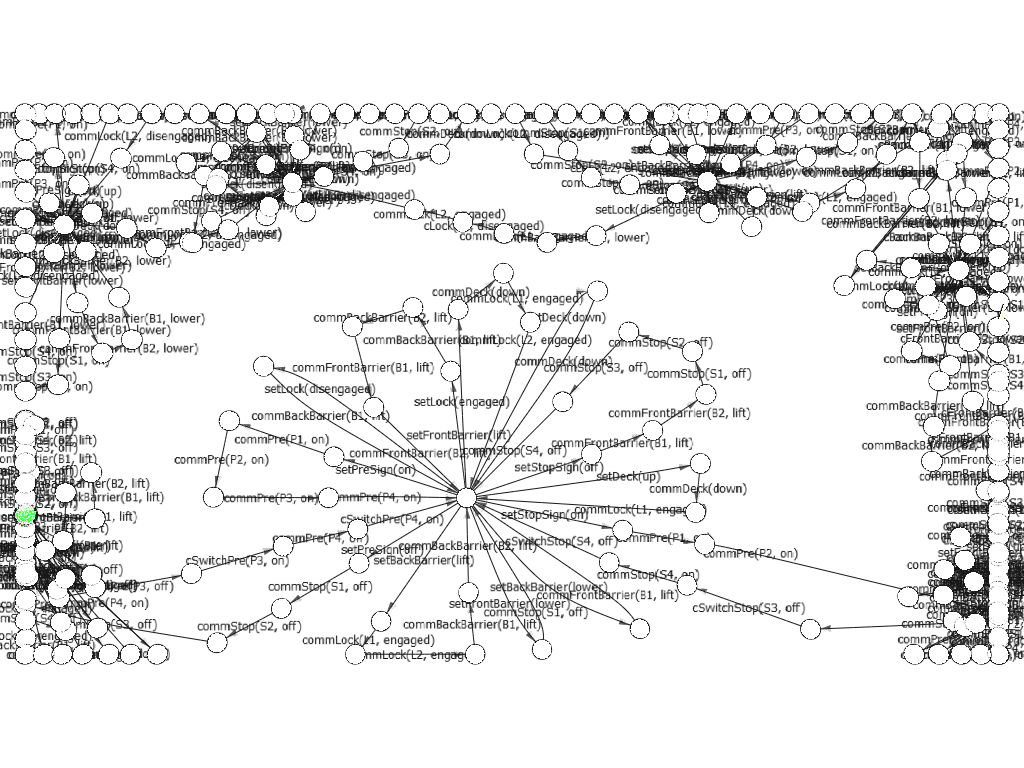
\includegraphics[width=\columnwidth]{Images/detail_graph.pdf}
\caption{Detailed representation of the model (pre sign node), depicting the check procedures for all possible commands.}%
\label{fig:detailed}
\end{figure}%
%

\newpage
